\chapter{Growth exponents for the Riemann zeta function}\label{zeta-growth-chapter}

\begin{definition}[Growth rate of zeta]\label{zeta-grow-def}  For any fixed $\sigma \in \R$, let $\mu(\sigma)$ denote the least possible (fixed) exponent for which one has the bound
    $$ |\zeta(\sigma+it)| \ll |t|^{\mu(\sigma)+o(1)}$$
    for all unbounded $t$.
\end{definition}

One can check that for each $\sigma$, the set of possible candidates for $\mu(\sigma)$ is closed (by underspill), non-empty, and bounded from below, so that $\mu(\sigma)$ is well-defined as a real number.  An equivalent definition without asymptotic notation, is that $\mu(\sigma)$ is the least real number such that for every $\eps>0$ there exists $C>0$ such that
$$ |\zeta(\sigma+it)| \leq C |t|^{\mu(\sigma)+\eps}$$
for all $t$ with $|t| \geq C$; equivalently, one has
$$ \mu(\sigma) = \limsup_{|t| \to \infty} \frac{\log |\zeta(\sigma+it)|}{\log|t|}.$$

\python{bound_mu}
\code{Bound_mu}

\begin{lemma}[Trivial bound]\label{zeta-grow-triv}\uses{zeta-grow-def}
    One has $\mu(\sigma)=0$ for all $\sigma \geq 1$.
\end{lemma}

\python{bound_mu}
\code{apply_trivial_mu_bound()}

\begin{proof}  Immediate from the absolute convergence of the Dirichlet series for both $\zeta(s)$ and $1/\zeta(s)$; see e.g., \cite[Theorem 1.9]{ivic}.
\end{proof}

\begin{lemma}[Convexity]\label{zeta-convex}\uses{zeta-grow-def}
$\mu$ is convex.
\end{lemma}

\python{bound_mu}
\code{bound_mu_convexity()}

\begin{proof} Immediate from the Phragm\'en--Lindel\"of principle; see e.g., \cite[\S A.8]{ivic}.
\end{proof}

\begin{lemma}[Functional equation]\label{zeta-functional}\uses{zeta-grow-def}
    One has $\mu(1-\sigma) = \mu(\sigma) + \sigma - 1/2$ for all $0 \leq \sigma \leq 1/2$.
\end{lemma}

\python{bound_mu}
\code{apply_functional_equation()}

\begin{proof}  Immediate from the functional equation for $\zeta$ and asymptotics of the Gamma function; see e.g., \cite[(1.23), (1.25)]{ivic}.
\end{proof}

\begin{lemma}[Left of critical strip]\label{zeta-left}\uses{zeta-grow-def}
    One has $\mu(\sigma)=1/2-\sigma$ for $\sigma \leq 0$.
\end{lemma}

\python{bound_mu}
\code{apply_trivial_mu_bound()}

\begin{proof}\uses{zeta-grow-triv, zeta-functional}  Immediate from Lemmas \ref{zeta-grow-triv}, \ref{zeta-functional}.
\end{proof}

\begin{lemma}[Convexity bounds]\label{zeta-convexity}\uses{zeta-grow-def}  One has $\max(0, 1/2-\sigma) \leq \mu(\sigma) \leq (1-\sigma)/2$ for $0 \leq \sigma \leq 1$.
\end{lemma}

\python{bound_mu}
\code{apply_trivial_mu_bound()}

\begin{proof}\uses{zeta-grow-triv, zeta-convex, zeta-left}  Immediate from Lemma \ref{zeta-grow-triv}, Lemma \ref{zeta-left}, and Lemma \ref{zeta-convexity}.
\end{proof}

\section{Connection with exponent pairs and dual exponent pairs}

\begin{lemma}[Connection with dual exponent pairs]\label{mu-beta}\label{zeta-grow-def, beta-def}  For any $1/2 \leq \sigma \leq 1$, one has
    $$ \mu(\sigma) \leq \sup_{0 \leq \alpha \leq 1/2} \beta(\alpha) - \alpha \sigma.$$
\end{lemma}

\begin{proof}\uses{auto}  Let $t$ be unbounded.  From the Riemann--Siegel formula (see \cite[Theorem 4.1]{ivic}) one has
    $$ \zeta(\sigma+it) \ll \left|\sum_{n \leq \sqrt{t/2\pi}} \frac{1}{n^{\sigma+it}}\right| + |t|^{1/2-\sigma} \left|\sum_{n \leq \sqrt{t/2\pi}} \frac{1}{n^{1-\sigma-it}}\right| + O(1).$$
From dyadic decomposition and Definition \ref{beta-def} (and Lemma \ref{auto}) one has for any fixed $\eps>0$ that
$$\sum_{t^\eps \leq n \leq \sqrt{t/2\pi}} \frac{1}{n^{\sigma+it}} \ll
|t|^{\sup_{\eps \leq \alpha \leq 1/2} \beta(\alpha) - \alpha \sigma + o(1)},$$
while from the triangle inequality one has the crude bound
$$\sum_{n < t^\eps} \frac{1}{n^{\sigma+it}} \ll |t|^\eps.$$
Combining the bounds and using underspill, we conclude that
$$\sum_{n \leq \sqrt{t/2\pi}} \frac{1}{n^{\sigma+it}} \ll
|t|^{\sup_{0 \leq \alpha \leq 1/2} \beta(\alpha) - \alpha \sigma + o(1)}.$$
A similar argument gives
$$\sum_{n \leq \sqrt{t/2\pi}} \frac{1}{n^{1-\sigma-it}} \ll
|t|^{\sup_{0 \leq \alpha \leq 1/2} \beta(\alpha) - \alpha (1-\sigma) + o(1)}$$
Since $\sigma \geq 1/2$ and $\alpha \leq 1/2$, one has $(1/2-\sigma) - \alpha(1-\sigma) \leq -\alpha \sigma$, and hence
$$ \zeta(\sigma+it) \ll
|t|^{\sup_{0 \leq \alpha \leq 1/2} \beta(\alpha) - \alpha \sigma + o(1)}$$
giving the claim.
\end{proof}

We remark that this inequality is morally an equality (indeed, it would be if one would restrict the model phases in Definition \ref{beta-def} to purely the logarithmic phase $u \mapsto \log u$).

The following form of Lemma \ref{mu-beta} is convenient for applications:

\begin{corollary}[Exponent pairs and $\mu$]\label{exp-pair-mu}\uses{exp-pair-def, zeta-grow-def} If $(k,\ell)$ is an exponent pair, then
$$ \mu(\ell-k) \leq k.$$
\end{corollary}

\python{bound_mu}
\code{exponent_pair_to_mu_bound(exp_pair)}

\begin{proof}\uses{mu-beta, beta-duality}  Immediate from Lemma \ref{mu-beta} and Lemma \ref{beta-duality}.  See also \cite[(7.57)]{ivic}.
\end{proof}

\begin{conjecture}[Lindel\"of hypothesis]\label{LH}\uses{zeta-grow-def} One has $\mu(1/2)=0$.
\end{conjecture}

\python{bound_mu}
\code{bound_mu_Lindelof()}

\begin{lemma}\label{exp-pair_implies_lindelof}\uses{exp-pair-conj, LH}  The exponent pair conjecture implies the Lindel\"of hypothesis.
\end{lemma}

\begin{proof}\uses{exp-pair-mu} Immediate from Corollary \ref{exp-pair-mu}.
\end{proof}

\begin{proposition}[Conjectured value of $\mu$]\label{mu-conj}\uses{zeta-grow-def, LH}  We have the lower bound
\begin{equation}\label{muh}
    \mu(\sigma) \geq \max\left(0, \frac{1}{2}-\sigma\right)
\end{equation}
for all $\sigma \in \R$, and equality holds everywhere in \eqref{muh} if and only if the Lindel\"of hypothesis holds.
\end{proposition}

We remark that this proposition explains why there are no further lower bounds on $\mu$ in the literature beyond \eqref{muh}; all the remaining known results revolve around upper bounds.

\begin{proof}\uses{zeta-grow-triv, zeta-left, zeta-convexity}  Clearly equality in \eqref{muh} implies the Lindel\"of hypothesis, while from the trivial bounds in Propositions \ref{zeta-grow-triv}, \ref{zeta-left} and convexity (Lemma \ref{zeta-convexity}) one we see that the Lindel\"of hypothesis implies the upper bound
$$     \mu(\sigma) \leq \max\left(0, \frac{1}{2}-\sigma\right)$$
for all $\sigma$.  So it suffices to establish the lower bound unconditionally.  By the functional equation (Proposition \ref{zeta-functional}) it suffices to do this for $\sigma \geq 1/2$; in fact by convexity it suffices to establish the claim when $1/2 < \sigma < 1$.  In this regime, the $L^2$ mean value theorem (see \cite[Theorem 1.11]{ivic}) gives
$$ \int_0^T |\zeta(\sigma+it)|^2\ dt \asymp T$$
for large $T$, giving the claim.
\end{proof}

\section{Known bounds on \texorpdfstring{$\mu$}{mu}}

\begin{theorem}[Historical bounds]\label{mu-hist}\uses{zeta-grow-def}  The upper bounds on $\mu(\sigma)$ given by Table \ref{mu-table} are known.
\end{theorem}

\textbf{TODO: supplement as many of these citations as possible with derivations from other exponents and relations in the database}

\begin{table}[ht]
\caption{Historical bounds on $\mu(\sigma)$ for $1/2 \le \sigma \le 1$, and the exponent pair generating them (if applicable).}
\centering
\renewcommand{\arraystretch}{1.2}
\begin{tabular}{|c|c|c|}
\hline
Reference & Results & Exponent pair \\
\hline
Hardy--Littlewood (1923) \cite{hardy_littlewood_1923} & $\mu(1/2) \le 1/6$ & (1/6, 2/3)\\
\hline
Walfisz (1924) \cite{walfisz_1924} & $\mu(1/2) \le 193/988$ & \\
\hline
Titchmarsh (1932) \cite{titchmarsh_van_1931} & $\mu(1/2) \leq 27/164$ & \\
\hline
Phillips (1933) \cite{phillips_zeta_1933} & $\mu(1/2) \leq 229/1392$ & \\
\hline
Titchmarsh (1942) \cite{titchmarsh_order_1942}  & $\mu(1/2) \leq 19/116$ & \\
\hline
Min (1949) \cite{min_on_1949} & $\mu(1/2) \leq 15/92$ & \\
\hline
Haneke (1962) \cite{haneke_verscharfung_1963} & $\mu(1/2) \leq 6/37$&  \\
\hline
Kolesnik (1973) \cite{kolesnik_1973} & $\mu(1/2) \leq 173/1067$ & \\
\hline
Kolesnik (1982) \cite{kolesnik_order_1982} & $\mu(1/2) \leq 35/216$ & \\
\hline
Kolesnik (1985) \cite{kolesnik_1985} & $\mu(1/2) \leq 139/858$ & \\
\hline
Bombieri--Iwaniec (1985) \cite{bombieri_order_1986} & $\mu(1/2) \leq 9/56$ & $(9/56, 1/2+9/56)$\\
\hline
Watt (1989) \cite{watt_exponential_1989} & $\mu(1/2) \leq 89/560$ & $(89/560, 1/2+89/560)$\\
\hline
Huxley--Kolesnik (1991) \cite{huxley_exponential_1991} & $\mu(1/2) \leq 17/108$ & $(17/108, 1/2+17/108)$\\
\hline
Huxley (1993) \cite{huxley_exponential_1993} & $\mu(1/2) \leq 89/570$ & $(89/570, 1/2+89/570)$\\
\hline
Huxley (1996) \cite{huxley_area_1996} & $\mu(1934/3655) \leq 6299/43860$ & \\
\hline
Sargos (2003) \cite{sargos_analog_2003} & $\mu(49/51) \leq 1/204$, $\mu(361/370) \leq 1/370$&  \\
\hline
Huxley (2005) \cite{huxley_exponential_2005} & $\mu(1/2) \leq 32/205$ & $(32/205, 1/2+32/205)$ \\
\hline
Lelechenko (2014) \cite{Lelechenko_linear_2014} & $\mu(3/5) \leq 1409/12170$, $\mu(4/5) \leq 3/71$& \\
\hline
Bourgain (2017) \cite{bourgain_decoupling_2017} & $\mu(1/2) \leq 13/84$ & $(13/84, 1/2+13/84)$ \\
\hline
Heath-Brown (2017) \cite{heathbrown_new_2017} & $\mu(\sigma) \le \frac{8}{63}\sqrt{15}(1 - \sigma)^{3/2}$ for $1/2 \le \sigma \le 1$& \\
\hline
Heath-Brown (2020) \cite{demeter_small_2020} & $\mu(11/15) \leq 1/15$& \\
\hline
\end{tabular}
\end{table}\label{mu-table}

\literature
\code{add_literature_bounds_mu()}

Some additional bounds are recorded in \cite{trudgian-yang} by combining various exponential sum estimates. 

\begin{theorem}\label{mu_est_thm}\cite[Theorems 2.4-2.6]{trudgian-yang}\uses{zeta-grow-def}
    We have
    \[
    \mu(\sigma) \le \begin{cases}
         (31 - 36\sigma)/84 , & \frac{1}{2} \leq\sigma < \frac{88225}{153852} = 0.5734\ldots, \\
         (220633 - 251324\sigma)/620612 , & \frac{88225}{153852} \leq\sigma < \frac{521}{796} = 0.6545\ldots, \\
         (1333 - 1508\sigma)/3825 , & \frac{521}{796} \leq\sigma < \frac{53141}{76066} = 0.6986\ldots, \\
         (405 - 454\sigma)/1202 , & \frac{53141}{76066} \leq\sigma < \frac{3620}{5119} = 0.7071\ldots, \\
         (49318855 - 52938216\sigma)/170145110 , & \frac{3620}{5119} \leq\sigma < \frac{52209}{69128} = 0.7552\ldots, \\
         (471957 - 502648\sigma)/1682490 , & \frac{52209}{69128} \leq\sigma < \frac{1389}{1736} = 0.8001\ldots, \\
         (2841 - 3016\sigma)/10316 , & \frac{1389}{1736} \leq\sigma < \frac{134765}{163248} = 0.8255\ldots, \\
         (859 - 908\sigma)/3214 , & \frac{134765}{163248} \leq\sigma < \frac{18193}{21906} = 0.8305\ldots, \\
         5(8707 - 9067\sigma)/180277 , & \frac{18193}{21906} \leq\sigma < \frac{249}{280} = 0.8892\ldots, \\
         (29 - 30\sigma)/130 , & \frac{249}{280} \leq\sigma \leq \frac{9}{10}.\\
    \end{cases}
    \]
    Furthermore, for $1/2 \le \sigma \le 1$, we have
\[
\mu(\sigma) \le \frac{2}{13}\sqrt{10}(1 - \sigma)^{3/2} = 0.4865\ldots(1 - \sigma)^{3/2},
\]
and
\[
\mu(\sigma) \le \frac{2}{3^{3/2}}(1 - \sigma)^{3/2} + \frac{103}{300}(1 - \sigma)^{2},\qquad \frac{117955}{118272} \le \sigma \le 1.
\]
\end{theorem}

\literature
\code{add_literature_bounds_mu()}

Additionally, the series of exponent pairs in \Cref{heath-brown_exp_pair_2017} imply the following bounds on $\mu(\sigma)$ close to $\sigma = 1$. 
\begin{theorem}[Heath-Brown \cite{heathbrown_new_2017} $\mu$ bounds]\label{hb_mu_bounds}\uses{exp-pair-def, exp-pair-mu, heath-brown_exp_pair_2017}
For any integer $k \ge 3$, one has
\[
\mu\left(1 - \frac{3 k^2 - 3 k + 2}{k(k - 1)^2(k + 2)}\right)\le \frac{2}{(k - 1)^2(k + 2)}.
\]
\end{theorem}
\begin{proof}
Follows from substituting \Cref{heath-brown_exp_pair_2017} into \eqref{exp-pair-mu}.
\end{proof}


The new exponent pairs in \Cref{new-exp-pair} may be used to obtain sharper bounds on $\mu(\sigma)$ in certain ranges. The current sharpest bounds on $\mu(\sigma)$ are recorded in \Cref{best-mu-table} and graphed in \Cref{fig:best_mu_bound}.


\begin{table}[ht]
\caption{Current sharpest known bound on $\mu(\sigma)$ for $1/2 \le \sigma \le 1$}
\centering
\renewcommand{\arraystretch}{2.2}
\begin{tabular}{|c|c|c|}
\hline
Upper bound on $\mu(\sigma)$ & Range of $\sigma$ & Reference \\
\hline
$\mu(\sigma) \leq \dfrac{31}{84} - \dfrac{3}{7}\sigma$ & $\dfrac{1}{2}\leq \sigma \leq \dfrac{88225}{153852} = 0.5734\ldots$ & \Cref{mu_est_thm}\\
\hline
$\mu(\sigma) \leq \dfrac{220633}{620612} - \dfrac{62831}{155153}\sigma$ & $\dfrac{88225}{153852}\leq \sigma \leq \dfrac{521}{796} = 0.6545\ldots$ & \Cref{mu_est_thm}\\
\hline
$\mu(\sigma) \leq \dfrac{1333}{3825} - \dfrac{1508}{3825}\sigma$ & $\dfrac{521}{796}\leq \sigma \leq \dfrac{53141}{76066} = 0.6986\ldots$ & \Cref{mu_est_thm}\\
\hline
$\mu(\sigma) \leq \dfrac{405}{1202} - \dfrac{227}{601}\sigma$ & $\dfrac{53141}{76066}\leq \sigma \leq \dfrac{454}{641} = 0.7082\ldots$ & \Cref{mu_est_thm}\\
\hline
$\mu(\sigma) \leq \dfrac{779}{2590} - \dfrac{423}{1295}\sigma$ & $\dfrac{454}{641}\leq \sigma \leq \dfrac{1744}{2411} = 0.7234\ldots$ & \Cref{new-exp-pair}, \Cref{exp-pair-mu}\\
\hline
$\mu(\sigma) \leq \dfrac{179}{622} - \dfrac{96}{311}\sigma$ & $\dfrac{1744}{2411}\leq \sigma \leq \dfrac{951057}{1298878} = 0.7322\ldots$ & \Cref{new-exp-pairs-2}, \Cref{exp-pair-mu}\\
\hline
$\mu(\sigma) \leq \dfrac{157319}{560830} - \dfrac{251324}{841245}\sigma$ & $\dfrac{951057}{1298878}\leq \sigma \leq \dfrac{1389}{1736} = 0.8001\ldots$ & \Cref{new-exp-pair}, \Cref{exp-pair-mu}\\
\hline
$\mu(\sigma) \leq \dfrac{2841}{10316} - \dfrac{754}{2579}\sigma$ & $\dfrac{1389}{1736}\leq \sigma \leq \dfrac{587779}{702192} = 0.8370\ldots$ & \Cref{mu_est_thm}\\
\hline
$\mu(\sigma) \leq \dfrac{1691}{6554} - \dfrac{890}{3277}\sigma$ & $\dfrac{587779}{702192}\leq \sigma \leq \dfrac{7441}{8695} = 0.8557\ldots$ & \Cref{new-exp-pair}, \Cref{exp-pair-mu}\\
\hline
$\mu(\sigma) \leq \dfrac{29}{130} - \dfrac{3}{13}\sigma$ & $\dfrac{7441}{8695}\leq \sigma \leq \dfrac{277}{300} = 0.9233\ldots$ & \Cref{new-exp-pair}, \Cref{hb_mu_bounds}\\
\hline
\begin{tabular}{@{}c@{}}
$\mu(\sigma) \leq \lambda\mu_n + (1 - \lambda)\mu_{n + 1}$ \\ $\mu_n = \dfrac{2}{(n - 1)^2(n + 2)}$ \\ $\lambda = (\sigma_{n + 1} - \sigma)/(\sigma_{n + 1} - \sigma_n)$ \end{tabular} & \begin{tabular}{@{}c@{}}$\sigma_n \leq \sigma \leq \sigma_{n + 1}$\\ $\sigma_n = 1 - \dfrac{3 n^2 - 3 n + 2}{n(n - 1)^2(n + 2)},\quad (n \ge 7)$\end{tabular} & \Cref{hb_mu_bounds} \\
\hline
\end{tabular}\label{best-mu-table}
\end{table}
\derived 
\code{compute_best_mu_bound()}

\begin{figure}
    \centering
    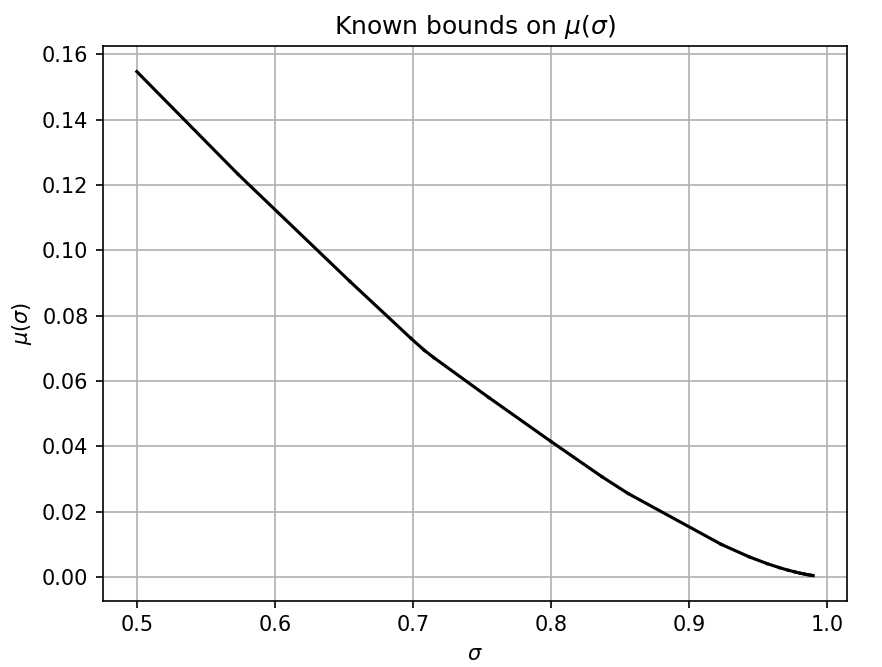
\includegraphics[width=0.5\linewidth]{chapter/mu_bound_plot.png}
    \caption{Current sharpest known bound on $\mu(\sigma)$ for $1/2 \le \sigma \le 1$.}
    \label{fig:best_mu_bound}
\end{figure}

\section{Connection to the Riemann hypothesis}

It is well known that the Riemann hypothesis implies the Lindel\"of hypothesis.  Here is a sharper version, essentially due to Backlund \cite{backlund}:

\begin{lemma}[Growth exponent and zeroes]  Let $1/2 \leq \sigma_0 < 1$ be fixed.  Then the assertion $\mu(\sigma_0)=0$ is equivalent to the assertion that for any fixed $\varepsilon>0$ and unbounded $T>0$, the number of zeroes $\sigma+it$ of the zeta function with $\sigma \geq \sigma_0+\varepsilon$ and $T \leq t \leq T+1$ is $o(\log T)$.
\end{lemma}

\begin{proof} This is a routine adaptation of Theorem 2 of \url{https://terrytao.wordpress.com/2015/03/01}.
\end{proof}
